% Filename : chapter_2.tex
\chapter{Review of Related Literature}
\label{sec:relatedlit}

\section{The effects of waiting in lines}

Spending time in physical queues imposes an economic and psychological cost on the individual \cite{chebat1993impact}. Not only does waiting in line elicit feelings of boredom, apathy, and frustration \cite{waitwhile2022survey}, but it can seriously impose on the time a person would have used to do other things. For example, the average American spends roughly 37 hours each year \cite{stone2012waiting}.

Long wait times can also be detrimental for businesses. Based on statistics cited by Brooke \citeyear{brooke2013ditch}, customers tend to react negatively to long wait times, becoming frustrated and abandoning lines if the wait goes for longer than expected, sometimes going so far as to actively avoid it in the future. Furthermore, as a customer’s evaluation of a product or service can be heavily influenced by the time they spent waiting to receive it, businesses have the imperative to minimize their customers’ perceived waiting time \cite{chebat1993impact}.

For these reasons, several different systems have been devised to make queueing more efficient and to mitigate the negative effects of waiting in line.

\section{Queue Management Systems}

\begin{figure}[h] %-- use [t] to place figure at top, [b] to place at the bottom, [h] for here
\centering
\caption{Comparison of physical and virtual queues}
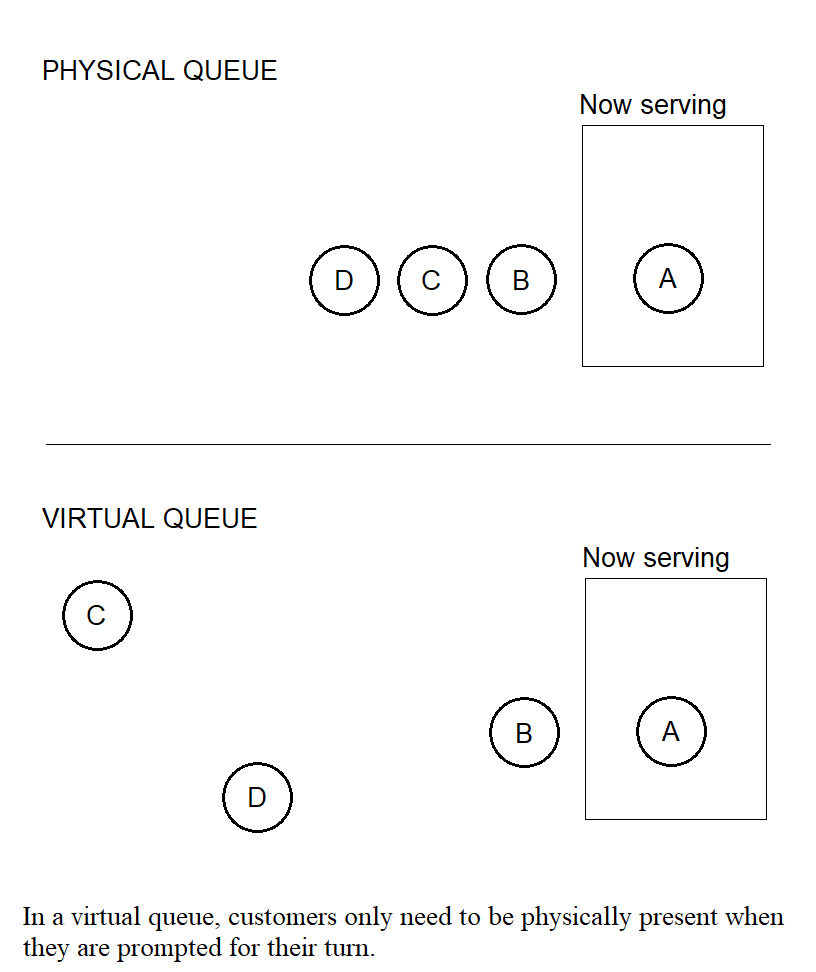
\includegraphics[scale=0.5]{QueueComparison.png}
\label{fig:queuecomparison}
\end{figure}


Queue management techniques exist to either improve the efficacy and service rate of a given queue, or make the time spent waiting within a queue more pleasant for the customer \cite{norman2008psychology}.

Among these techniques are virtual queue management systems \cite{mwangi2013reducing}. These are a specific form of queue management system that places customers in a virtual waiting line \cite{thamrin2020qmatic}, removing the need to be physically present while waiting in a line \cite{waitwhile2022survey}. As seen in figure \ref{fig:queuecomparison}, this offers a lot of convenience to customers, as they are not confined to a specific area and are free to use their waiting time as they see fit.

The benefits of virtual queueing apply to both customers and businesses \cite{thamrin2020qmatic}, streamlining communication between both parties, reducing perceived waiting times, improving customer flow management and worker efficiency, and increasing customer satisfaction. Furthermore, the non-physical nature of virtual queues also make it much easier to help reduce the spread of communicable diseases, a problem which is worth consideration during a pandemic.

Compared to other queueing management systems, virtual queues are observed to have a stronger positive effect in reducing wait delays and improving customer experiences \cite{mwangi2013reducing}.

In a survey conducted by Waitwhile \cite{waitwhile2022survey} that compares customer perceptions towards virtual and physical queueing, almost 70\% of respondents prefer virtual over physical queueing, and nearly 71\% of respondents were more willing to wait for longer periods of time in a virtual queue.

\section{Review of Similar Solutions}

There exist several implementations of virtual queues and similar systems intended to offer virtual solutions to physical queues. Such solutions are frequently implemented by establishments such as banks, hospitals, and payment centers in the form of ticketing systems, where customers are instructed to take a number that represents their position in line. Once they have their number, they are to wait within a designated space until their number is reached and they are prompted for their turn.

In virtual queues like the Fastpass system that Disney theme parks implement for their own attractions \cite{cope2011innovative}. This allows the parks to improve customer satisfaction and obtain additional revenue by allowing their guests to spend money on other attractions and services while they wait for their designated time.

Although ticketing systems are effective at reducing the problems associated with waiting in physical lines, customers are still confined to waiting areas.

There are also a number of software systems that fulfill a similar purpose as the intended research project.

	Mwai \citeyear{mwaivirtual} developed a cloud and mobile based system for queue management. Using Android Studio to develop their mobile application, and Wampserver 2.1 to develop the web server with a MySQL database. Data exchange between the application and the web server was handled by Firebase Cloud Storage. The resulting system allows for customers to enter virtual queues through online tokens or physical kiosks and be notified through their mobile devices when it is their turn.

One mobile application available on the Google Store, \textit{ApnaQ} \citeyear{appnaq}, provides a system for users to maintain and manage virtual queues, but is unavailable for users within the Philippines.

\textit{Queue: Virtual Queue Management} \citeyear{virtualqueueapp} is a free application that provides a cloud-based service for creating and implementing virtual queues created by users of the application. However, outside of the system used for implementing virtual queues, the application does not offer any additional features to its users.

\textit{Waitwhile} \citeyear{waitwhile} is an advanced application that provides a virtual queue service that businesses can use to set up queues and waitlists for their customers. Their service allows customers to join a waitlist through various methods and will provide reminders through their medium of choice. It also uses machine learning technology to manage queue capacity and estimate waiting times. Although WaitWhile offers a free option for businesses, a paid subscription is necessary to provide more than two reminders and handle more than one location.

\textit{Qmatic} \citeyear{qmatic} is a company that offers customer management services and solutions to their partners. Virtual queues are among the solutions they provide, where customers are able to join queues through various methods such as links, QR codes, or self-service kiosks. Once they are in a queue, customers are able to monitor their progress within the queue in real time, and receive notifications when they are next in line. While this service provides a suitable amount of additional features to improve customers’ experience of waiting in line, these services are only available to businesses that enter into a partnership with the company, which comes with additional fees.

Therefore, it is established that in order to create the best product for the intended user group discussed in Chapter 1, Section 1.5, the application project should be readily available for and affordable to the widest possible demographic, and should also provide an adequate number of features to improve the users’ experience using the application.
